\documentclass[conference]{IEEEtran}
\IEEEoverridecommandlockouts
% The preceding line is only needed to identify funding in the first footnote. If that is unneeded, please comment it out.
\usepackage{cite}
\usepackage{amsmath,amssymb,amsfonts}
\usepackage{algorithmic}
\usepackage{graphicx}
\usepackage{textcomp}
\usepackage{subcaption}
\usepackage{xcolor}
\def\BibTeX{{\rm B\kern-.05em{\sc i\kern-.025em b}\kern-.08em
    T\kern-.1667em\lower.7ex\hbox{E}\kern-.125emX}}
\begin{document}

\title{A fuzzy inference model for cancer risk prediction\\
}

\author{\IEEEauthorblockN{María Camila Vásquez Correa}
\IEEEauthorblockA{\textit{Mathematics department} \\
\textit{Universidad EAFIT}\\
Medellín, Colombia \\
mvasqu49@eafit.edu.co}
}

\maketitle

\begin{abstract}
In this article is presented a model of fuzzy inference in cancer risk, with three variables of support: habits, heritage and age. The model is tested in various scenarios with different methods for logical operations and defuzzification.
\end{abstract}

\begin{IEEEkeywords}
Fuzzy, Inference, FIS, cancer, risk.
\end{IEEEkeywords}

\section{Introduction}
Cancer is the leading life-threatening disease for people in today’s world. Although cancer formation is different and doctors often cannot explain why one person develops cancer and another does not, research shows that certain risk factors increase the chance that a person will develop cancer \cite{COGGON20051434}. Cancer prevention through consequent screening programs, early discovery and timely, improved and diversified means of treatment are usually the most successful ways to reduce mortality. \\

Where uncertainty exists such as in the medical
field, fuzzy logic could play an important role in making decisions. Fuzzy logic is the science of reasoning, thinking, and inference that recognizes and uses the real world phenomenon that every- thing is a matter of degree. In the simplest terms, fuzzy logic theory is an extension of binary theory that does not use crisp definitions and distinctions.
Instead of assuming everything must be
defined crisply into black and white (binary view), fuzzy logic is a method that captures and uses the concept of fuzziness in a computationally effective manner \cite{Zadeh1996}. \\

The objective of this work is to design and implement a fuzzy inference model and to analyze its results in predicting the risk of cancer in several cases. We suppose then that three variables are somehow enough to describe a possibility of developing cancer and we test the model in different scenarios.

The rest of the paper is organized as follows: first, there is a review of the current work regarding the topic. Second, there is an explanation of the methodology that is going to be used. Then the results of the model are presented and finally some conclusions are derived from the work.

\section{Literature review}
Many authors have addressed the problem of an early diagnose of cancer using fuzzy models that incorporate characteristics of the patients. And although these models share a common core, they are very different and approach the problem from different perspectives. \\

Most of the existing models try to model the risk of developing cancer in a specific organ. Such models include: breast cancer (\cite{Balanica2011}, \cite{Buyukavcu2016},
\cite{Gayathri2016},
\cite{Khezri2014},
\cite{Latha2013},
\cite{Papageorgiou2015},
\cite{Shleeg2013},
\cite{Subramanian2015},
\cite{Tatari2012},
\cite{Yilmaz2011}), prostate cancer (\cite{Benecchi2006},
\cite{Cosma2016}), oral cancer (\cite{Dom2012}), gastric cancer (\cite{Safdari2018}), colon cancer (\cite{Brand2006}) and lung cancer (\cite{Ylmaz2016}). However, there exists some other models that try to asses the risk of developing any kind of cancer, such as \cite{Atnccedil2012} and \cite{Dudek2012}. \\

They vary also in the type of fuzzy model that is being used. Most of them are a fuzzy inference model of type Mandani (\cite{Balanica2011}, \cite{Dudek2012}, \cite{Brand2006}, \cite{Gayathri2016}, \cite{Khezri2014}, \cite{Latha2013}, \cite{Safdari2018},
\cite{Yilmaz2011}) or Sugeno (\cite{Atnccedil2012},
\cite{Shleeg2013}). Though neural fuzzy models (\cite{Benecchi2006},
\cite{Dom2012},
\cite{Cosma2016},
\cite{Ylmaz2016}), fuzzy cognitive maps (\cite{Buyukavcu2016},
\cite{Papageorgiou2015},
\cite{Subramanian2015}) and fuzzy probabilistic models (\cite{Tatari2012}) have been used in this field. \\

The way of modelling the characteristics of the patients is very similar in some models. They include hereditary characteristics, like the genetic history; lifestyle characteristics, such as the nutrition, the smoking habits, the body mass index and physical activity; biological factors like hormones, pre-existing tumors and cell conditions. Finally, they consider socio-demographic factors, such as age and gender. \\

In this work we aim to use three of the main groups of characteristics, socio-demographic, lifestyle and hereditary, to propose a Mandani fuzzy inference model for predicting the risk of developing any type of cancer.

\section{Methodology}
The model used to carry out this work is described in detail below:
\subsection{Variables}
\begin{itemize}
  \item $u_1$: Quality of the habits (lifestyle).
  \item $u_2$: Quality of the genetic heritage. A good genetic heritage implies rare or non history of cancer.
  \item $u_3$: Age of the person.
  \item $y$: Risk of developing cancer.
\end{itemize}
\subsection{Speech Universe}
\begin{itemize}
  \item $u_1 \in \mathbb{Z} \cap [0,10]$: Being 0 the worst habits and 10 the best.
  \item $u_2  \in \mathbb{Z} \cap [0,10]$: Being 0 the worst heritage and 10 the best.
  \item $u_3  \in \mathbb{Z} \cap [0,90]$.
  \item $y  \in \mathbb{R} \cap [0,100]$.
\end{itemize}
\subsection{Linguistic categories}
\begin{itemize}
  \item $u_1$: Poor, medium and high quality.
  \item $u_2$: Poor, medium and high quality.
  \item $u_3$: Young, medium and old.
  \item $y$: High, medium and low.
\end{itemize}

\subsection{Membership functions}
In the Figure~\ref{fig:mem} are shown the respective membership functions for each one of the linguistic categories. They are defined as:
\begin{itemize}
    \item $u_1$:
    \begin{itemize}
        \item \textit{Poor}: $trapezoid(x;0,0,2,4)$
        \item \textit{Medium}: $gauss(x;5,1)$
        \item \textit{High}: $trapezoid(x;6,8,10,10)$
    \end{itemize}
    \item $u_2$:
    \begin{itemize}
        \item \textit{Poor}: $sigmoid(x;3,-2.64)$
        \item \textit{Medium}: $gauss(x;5,1)$
        \item \textit{Low}: $sigmoid(x;7,2.64)$
    \end{itemize}
    \item $u_3$:
    \begin{itemize}
        \item \textit{Poor}: $sigmoid(x;30,-0.53)$
        \item \textit{Medium}: $gauss(x;50,15.\bar{33})$
        \item \textit{Low}: $sigmoid(x;70,0.264)$
    \end{itemize}
    \item $y$:
    \begin{itemize}
        \item \textit{Poor}: $sigmoid(x;30,-0.264)$
        \item \textit{Medium}: $gauss(x;50,10)$
        \item \textit{Low}: $sigmoid(x;70,0.264)$
    \end{itemize}
\end{itemize}
\begin{figure*}[t!]
    \centering
    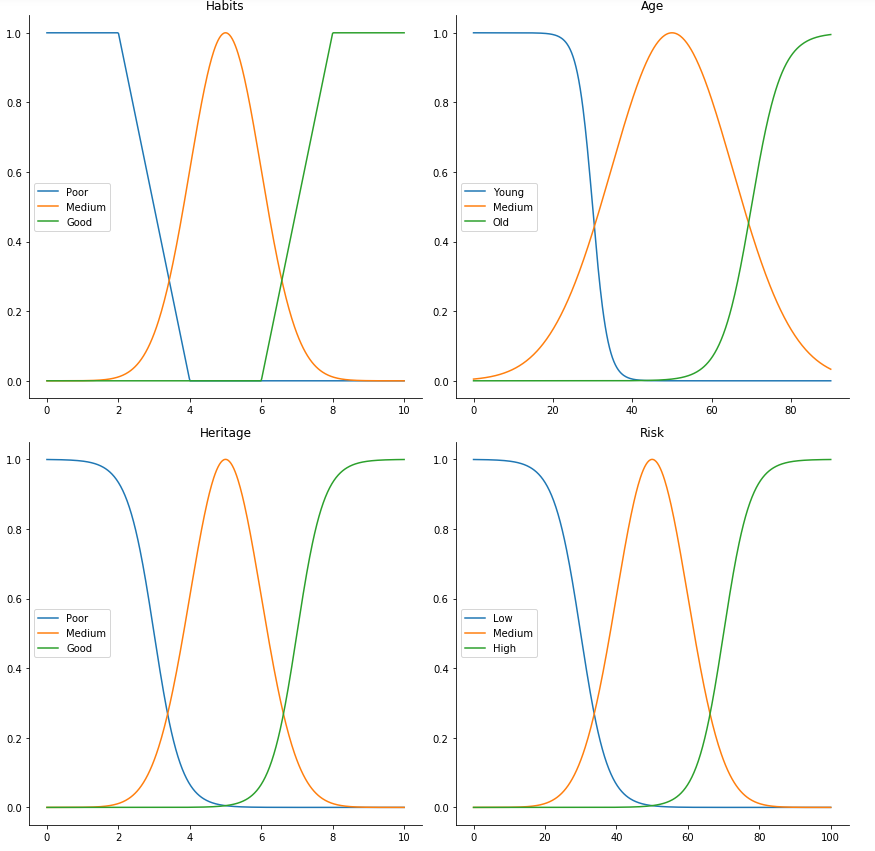
\includegraphics[scale = 0.6]{figures/mem.PNG}
    \caption{Membership functions}
    \label{fig:mem}
\end{figure*}

\subsection{Rule base}
\begin{itemize}
\item If [$u_1$ Poor] and [$u_2$ Poor] and [$u_3$ Low] then [$y$ Medium]
\item If [$u_1$ Poor] and [$u_2$ Poor] and [$u_3$ Medium] then [$y$ Medium]
\item If [$u_1$ Poor] and [$u_2$ Poor] and [$u_3$ High] then [$y$ High]
\item If [$u_1$ Poor] and [$u_2$ Medium] and [$u_3$ Low] then [$y$ Low]
\item If [$u_1$ Poor] and [$u_2$ Medium] and [$u_3$ Medium] then [$y$ Medium]
\item If [$u_1$ Poor] and [$u_2$ Medium] and [$u_3$ High] then [$y$ High]
\item If [$u_1$ Poor] and [$u_2$ High] and [$u_3$ Low] then [$y$ Low]
\item If [$u_1$ Poor] and [$u_2$ High] and [$u_3$ Medium] then [$y$ Low]
\item If [$u_1$ Poor] and [$u_2$ High] and [$u_3$ High] then [$y$ Medium]
\item If [$u_1$ Medium] and [$u_2$ Poor] and [$u_3$ Low] then [$y$ Medium]
\item If [$u_1$ Medium] and [$u_2$ Poor] and [$u_3$ Medium] then [$y$ High]
\item If [$u_1$ Medium] and [$u_2$ Poor] and [$u_3$ High] then [$y$ High]
\item If [$u_1$ Medium] and [$u_2$ Medium] and [$u_3$ Low] then [$y$ Low]
\item If [$u_1$ Medium] and [$u_2$ Medium] and [$u_3$ Medium] then [$y$ Medium]
\item If [$u_1$ Medium] and [$u_2$ Medium] and [$u_3$ High] then [$y$ High]
\item If [$u_1$ Medium] and [$u_2$ High] and [$u_3$ Low] then [$y$ Low]
\item If [$u_1$ Medium] and [$u_2$ High] and [$u_3$ Medium] then [$y$ Low]
\item If [$u_1$ Medium] and [$u_2$ High] and [$u_3$ High] then [$y$ Medium]
\item If [$u_1$ High] and [$u_2$ Poor] and [$u_3$ Low] then [$y$ Medium]
\item If [$u_1$ High] and [$u_2$ Poor] and [$u_3$ Medium] then [$y$ Medium]
\item If [$u_1$ High] and [$u_2$ Poor] and [$u_3$ High] then [$y$ Medium]
\item If [$u_1$ High] and [$u_2$ Medium] and [$u_3$ Low] then [$y$ Low]
\item If [$u_1$ High] and [$u_2$ Medium] and [$u_3$ Medium] then [$y$ Low]
\item If [$u_1$ High] and [$u_2$ Medium] and [$u_3$ High] then [$y$ Medium]
\item If [$u_1$ High] and [$u_2$ High] and [$u_3$ Low] then [$y$ Low]
\item If [$u_1$ High] and [$u_2$ High] and [$u_3$ Medium] then [$y$ Low]
\item If [$u_1$ High] and [$u_2$ High] and [$u_3$ High] then [$y$ Low]
\end{itemize}

\section{Results}
The rule base was implemented using a Mamdani and the aggregation method max min. Additionally, three methods of deffuzification methods (Centroid of the area, bisector of the area and mean of maximum) and two T-norms used for the activation of the rules (Minimum and product) with their respective S-rule (Maximum and sum - product). The implementation was made on Python using the module scikit-fuzzy. \\

\subsection{Response surfaces}
In this section, are described and shown some of the response surfaces of the model. 
\subsection{Test cases}
Then, three test cases were evaluated with each one of the T-norms and the defuzzification methods:
\begin{itemize}
    \item A healthy person, medium age, with good heritage. (habits = 7, age = 20, heritage = 8)
    \item A non-healthy young person with poor heritage. (habits = 4 age = 10 heritage = 3)
    \item A healthy old person with poor heritage. (habits = 10 age = 75 heritage = 3)
\end{itemize}

\subsubsection{Test case 1}
In the Figures~\ref{fig:testcase1min} and \ref{fig:testcase1prod} are shown the results for the first case, an ideal case, in which a person is not expected to develop cancer soon. The final risk of cancer is 15, 18 or 19, depending on the defuzzification method and the norm used. However, these values are not far apart from each other and indicate that the person is not in immediate danger, a reasonable conclusion taking into account the fact that they have healthy habits and a good genetic heritage. We see that, in this case, the minimum norm produces a higher output than the product norm, and the mean of maximum defuzzification method always produces the lowest output for the risk.
\begin{figure*}[ht]
\begin{subfigure}{.5\textwidth}
  \centering
  % include first image
  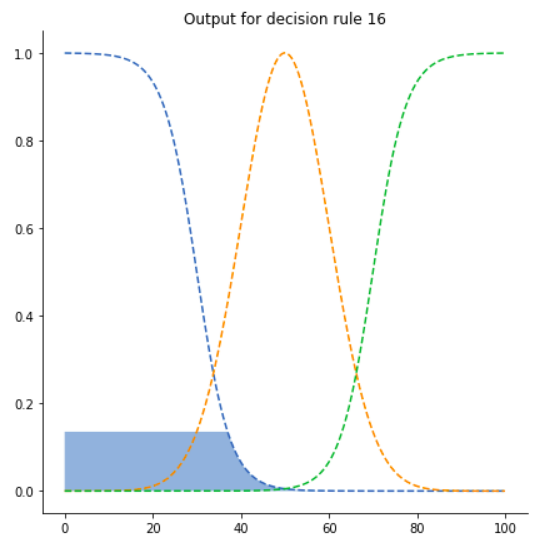
\includegraphics[width=.8\linewidth]{figures/first/min1.png}  
  \caption{Output for decision rule 16 with the T-norm minimum.}
  \label{fig:1min1}
\end{subfigure}
\begin{subfigure}{.5\textwidth}
  \centering
  % include second image
  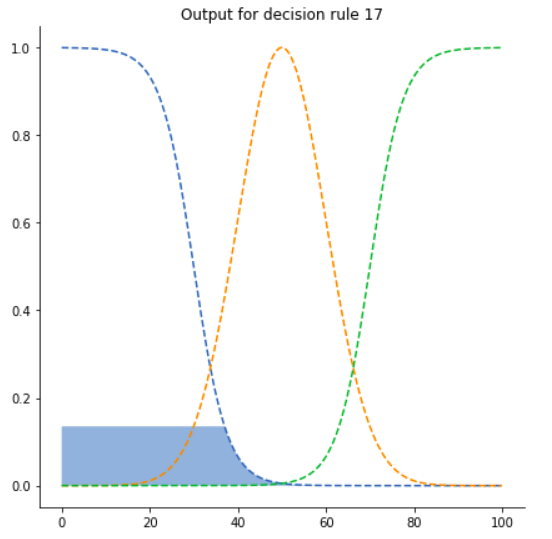
\includegraphics[width=.8\linewidth]{figures/first/min2.png}  
  \caption{Output for decision rule 17 with the T-norm minimum.}
  \label{fig:1min2}
\end{subfigure}
\begin{subfigure}{.5\textwidth}
  \centering
  % include second image
  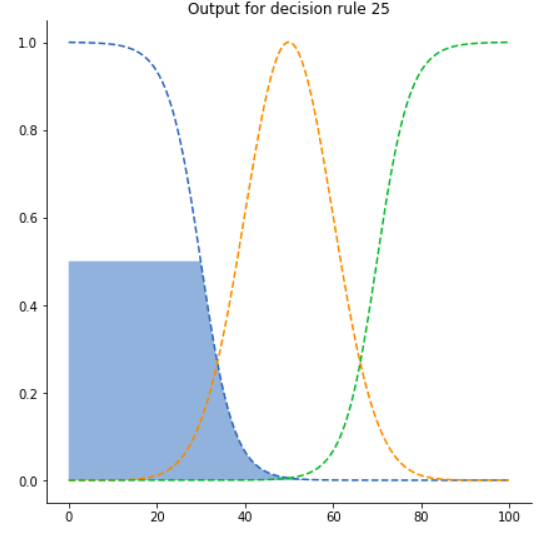
\includegraphics[width=.8\linewidth]{figures/first/min3.png}  
  \caption{Output for decision rule 25 with the T-norm minimum.}
  \label{fig:1min3}
\end{subfigure}
\begin{subfigure}{.5\textwidth}
  \centering
  % include second image
  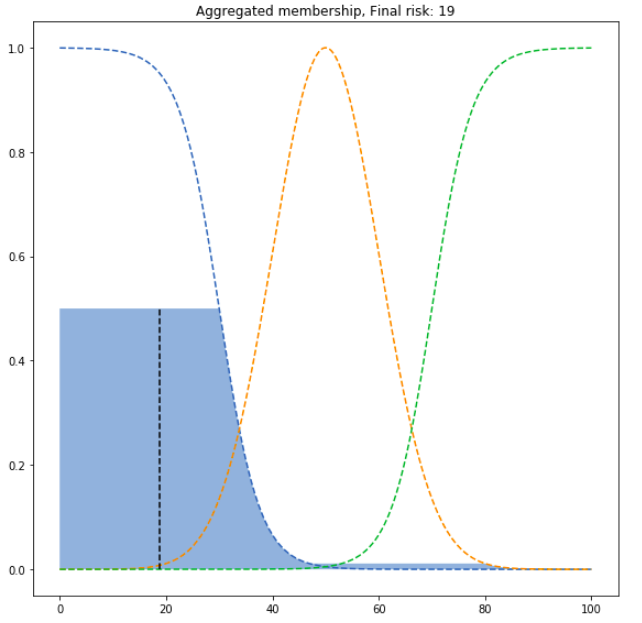
\includegraphics[width=.8\linewidth]{figures/first/min-centroid.png}  
  \caption{Final aggregation result with the centroid method for defuzzification.}
  \label{fig:1min-centroid}
\end{subfigure}
\begin{subfigure}{.5\textwidth}
  \centering
  % include second image
  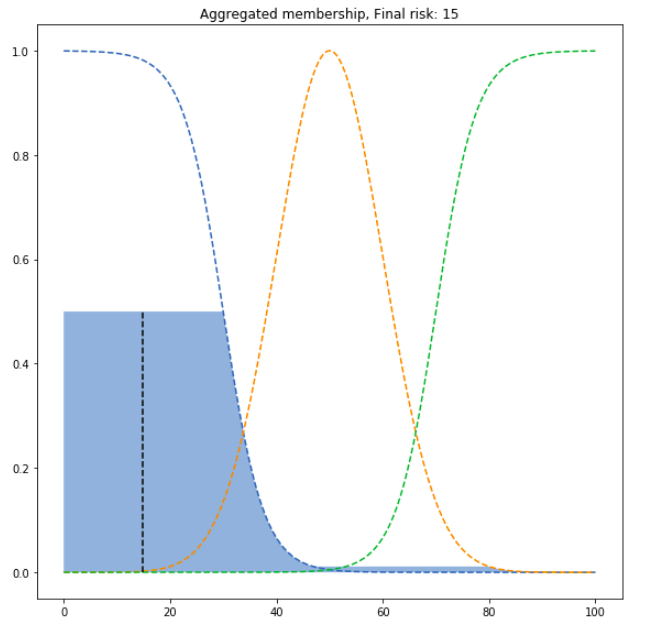
\includegraphics[width=.8\linewidth]{figures/first/min-mom.png}  
  \caption{Final aggregation result with the mean of maximum method for defuzzification.}
  \label{fig:1min-mom}
\end{subfigure}
\begin{subfigure}{.5\textwidth}
  \centering
  % include second image
  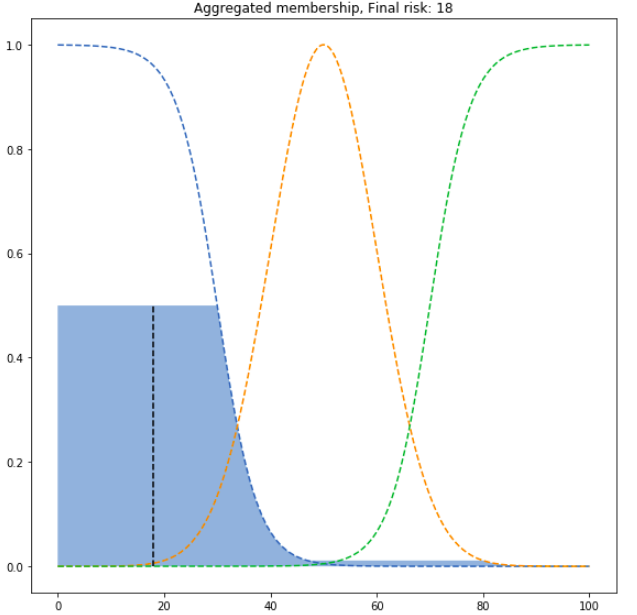
\includegraphics[width=.8\linewidth]{figures/first/min-bisector.png}  
  \caption{Final aggregation result with the bisector method for defuzzification.}
  \label{fig:1min-bisector}
\end{subfigure}
\caption{Results for test case 1 using the T-norm minimum.}
\label{fig:testcase1min}
\end{figure*}

\begin{figure*}[ht]
\begin{subfigure}{.5\textwidth}
  \centering
  % include first image
  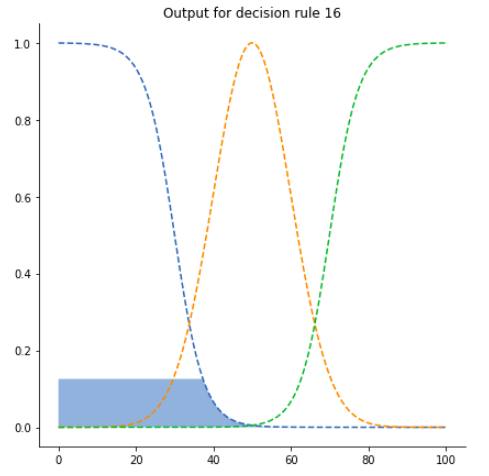
\includegraphics[width=.8\linewidth]{figures/first/prod1.png}  
  \caption{Output for decision rule 16 with the T-norm product.}
  \label{fig:1prod1}
\end{subfigure}
\begin{subfigure}{.5\textwidth}
  \centering
  % include second image
  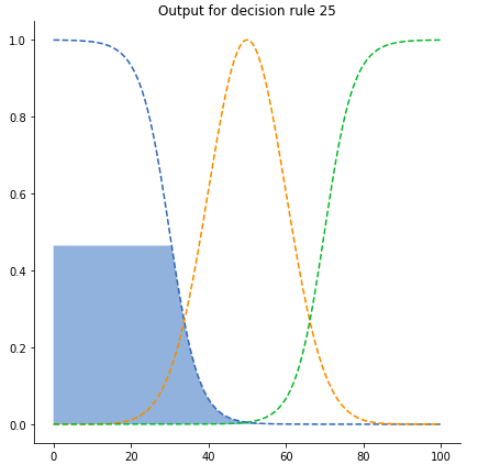
\includegraphics[width=.8\linewidth]{figures/first/prod2.png}  
  \caption{Output for decision rule 17 with the T-norm product.}
  \label{fig:1prod2}
\end{subfigure}
\begin{subfigure}{.5\textwidth}
  \centering
  % include second image
  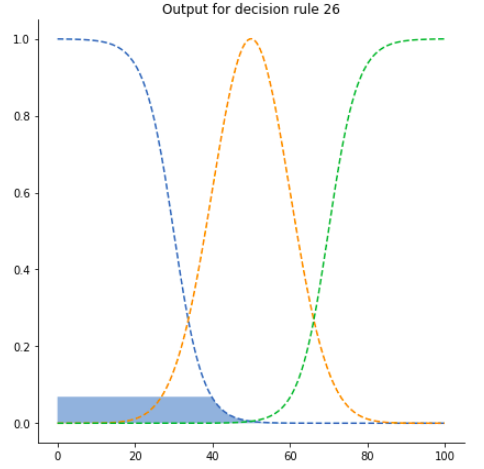
\includegraphics[width=.8\linewidth]{figures/first/prod3.png}  
  \caption{Output for decision rule 25 with the T-norm product.}
  \label{fig:1prod3}
\end{subfigure}
\begin{subfigure}{.5\textwidth}
  \centering
  % include second image
  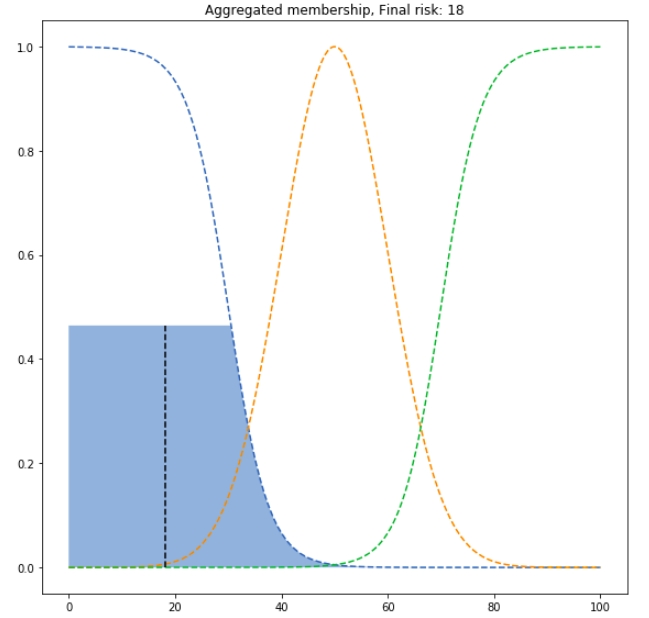
\includegraphics[width=.8\linewidth]{figures/first/prod-centroid.png}  
  \caption{Final aggregation result with the centroid method for defuzzification.}
  \label{fig:1prod-centroid}
\end{subfigure}
\begin{subfigure}{.5\textwidth}
  \centering
  % include second image
  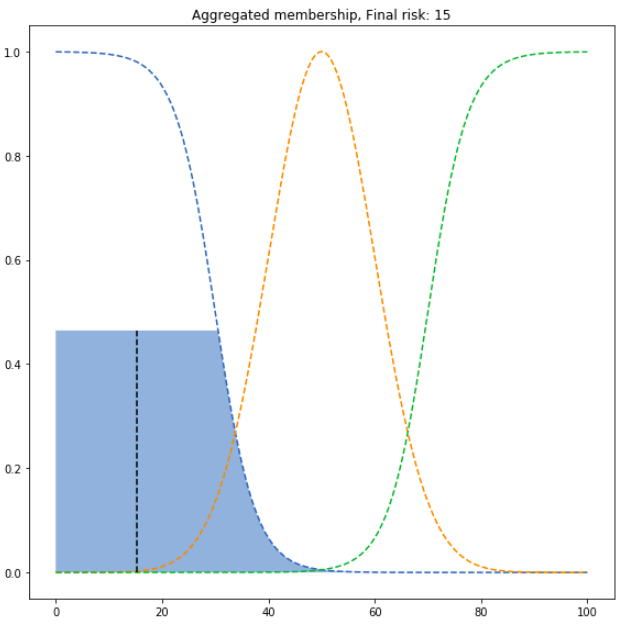
\includegraphics[width=.8\linewidth]{figures/first/prod-mom.png}  
  \caption{Final aggregation result with the mean of maximum method for defuzzification.}
  \label{fig:1prod-mom}
\end{subfigure}
\begin{subfigure}{.5\textwidth}
  \centering
  % include second image
  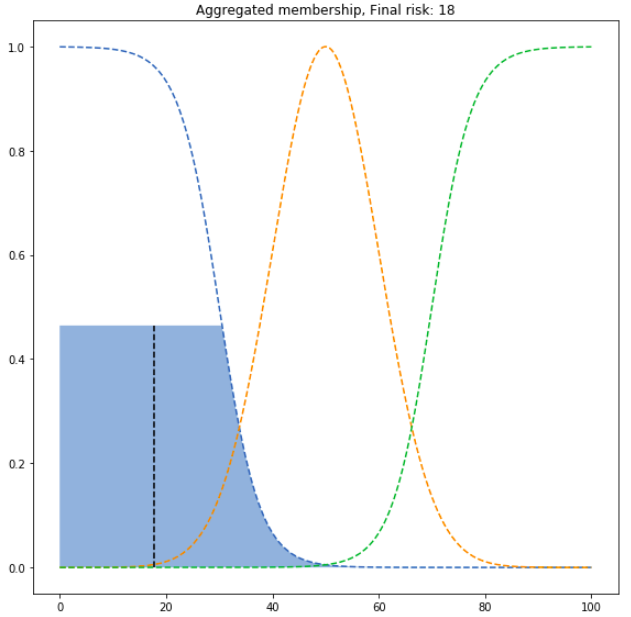
\includegraphics[width=.8\linewidth]{figures/first/prod-bisector.png}  
  \caption{Final aggregation result with the bisector method for defuzzification.}
  \label{fig:1prod-bisector}
\end{subfigure}
\caption{Results for test case 1 using the T-norm product.}
\label{fig:testcase1prod}
\end{figure*}

\subsubsection{Test case 2}
In the Figures~\ref{fig:testcase2min} and \ref{fig:testcase2prod} are shown the results for the second test case, in which a person is really young but has a bad heritage, that is, maybe they have some history of cancer in the family. Also, they do not have really good habits. We can see that the model takes all into account and for different rules has medium, low or high risk, each one for their habits, age and genetic heritage. The final risk is 45, 47 or 50, depending on the defuzzification method, but they do not vary with the norm used for the rule base. In this case, the mean of maximum produces the highest output of the risk. This is a case in which we identify that, even though the habits and the heritage have a bad quality, the fact that the patient is really young makes the risk medium. One can argue that the intuitive probability of this happening is really low, but cases show that really young people can develop cancer due to genetic factors.
\begin{figure*}[ht]
\begin{subfigure}{.5\textwidth}
  \centering
  % include second image
  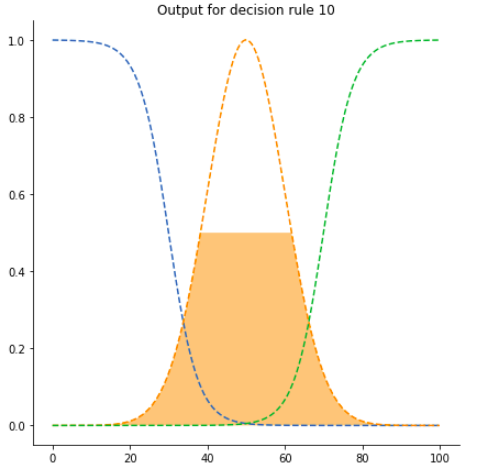
\includegraphics[width=.8\linewidth]{figures/second/min1.png}  
  \caption{Output for decision rule 10 with the T-norm minimum.}
  \label{fig:2min1}
\end{subfigure}
\begin{subfigure}{.5\textwidth}
  \centering
  % include second image
  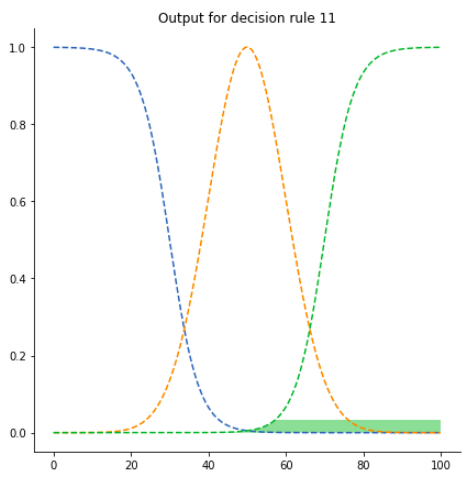
\includegraphics[width=.8\linewidth]{figures/second/min2.png}  
  \caption{Output for decision rule 11 with the T-norm minimum.}
  \label{fig:2min2}
\end{subfigure}
\begin{subfigure}{.5\textwidth}
  \centering
  % include second image
  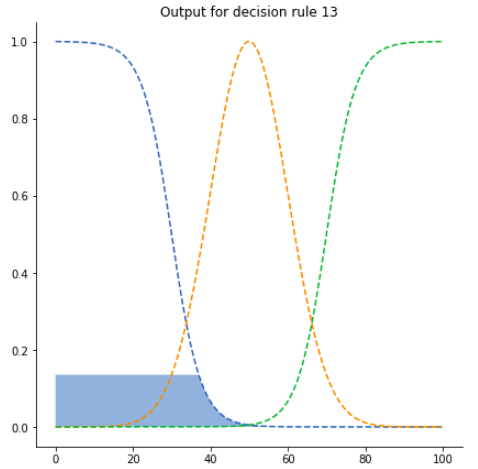
\includegraphics[width=.8\linewidth]{figures/second/min3.png}  
  \caption{Output for decision rule 13 with the T-norm minimum.}
  \label{fig:2min3}
\end{subfigure}
\begin{subfigure}{.5\textwidth}
  \centering
  % include second image
  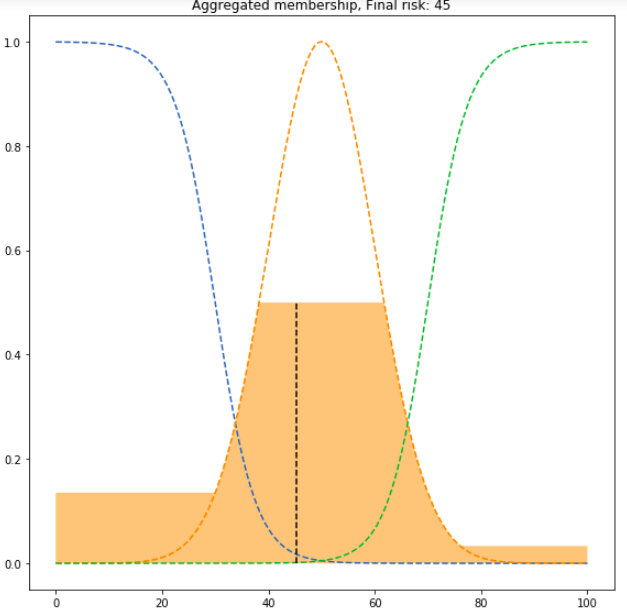
\includegraphics[width=.8\linewidth]{figures/second/min-centroid.png}  
  \caption{Final aggregation result with the centroid method for defuzzification.}
  \label{fig:2min-centroid}
\end{subfigure}
\begin{subfigure}{.5\textwidth}
  \centering
  % include second image
  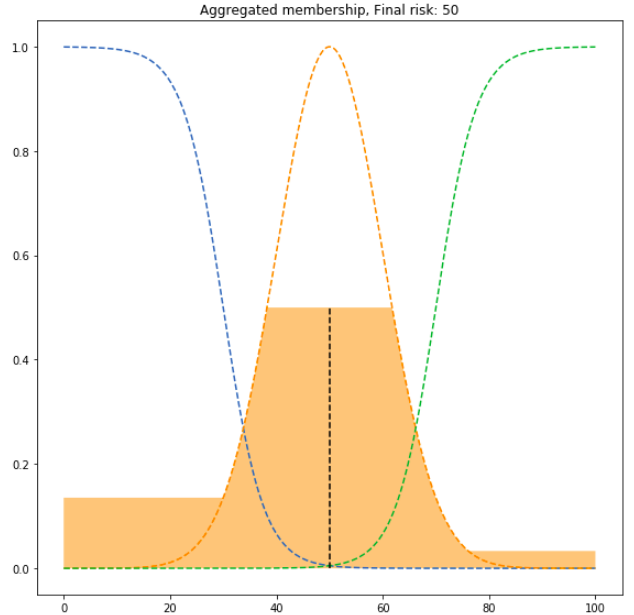
\includegraphics[width=.8\linewidth]{figures/second/min-mom.png}  
  \caption{Final aggregation result with the mean of maximum method for defuzzification.}
  \label{fig:2min-mom}
\end{subfigure}
\begin{subfigure}{.5\textwidth}
  \centering
  % include second image
  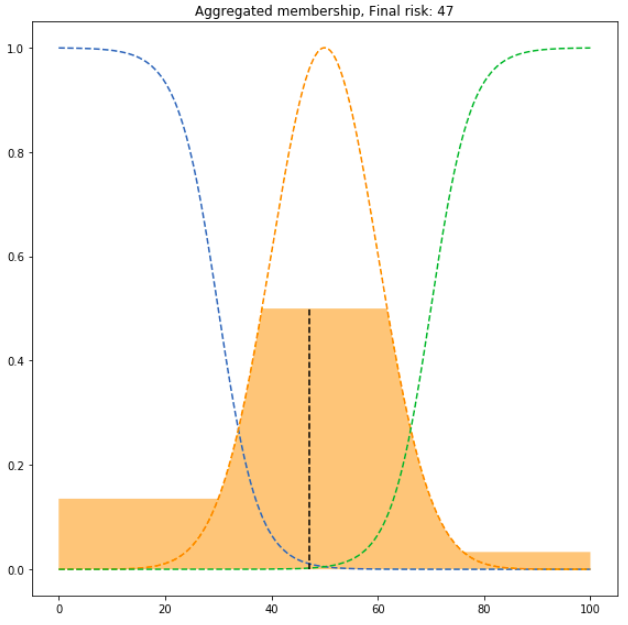
\includegraphics[width=.8\linewidth]{figures/second/min-bisector.png}  
  \caption{Final aggregation result with the bisector method for defuzzification.}
  \label{fig:2min-bisector}
\end{subfigure}
\caption{Results for test case 2 using the T-norm minimum.}
\label{fig:testcase2min}
\end{figure*}

\begin{figure*}[ht]
\begin{subfigure}{.5\textwidth}
  \centering
  % include second image
  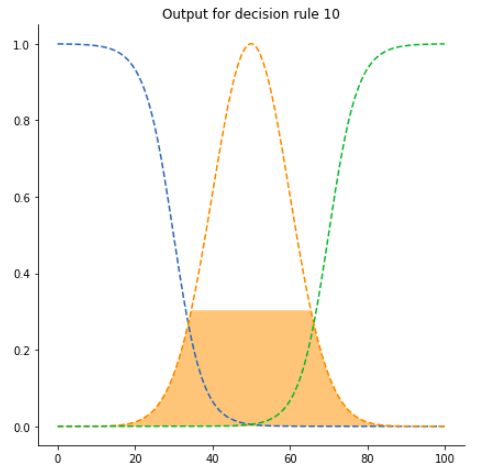
\includegraphics[width=.8\linewidth]{figures/second/prod1.png}  
  \caption{Output for decision rule 10 with the T-norm product.}
  \label{fig:2prod1}
\end{subfigure}
\begin{subfigure}{.5\textwidth}
  \centering
  % include second image
  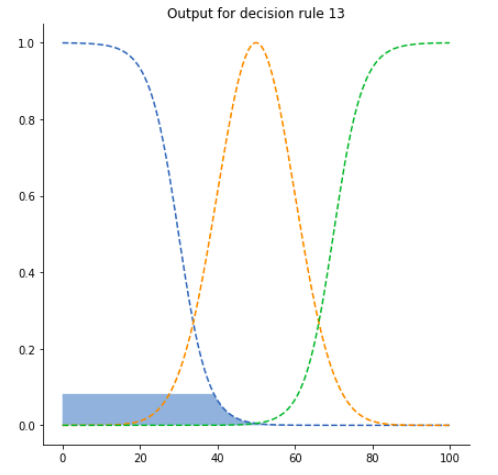
\includegraphics[width=.8\linewidth]{figures/second/prod2.png}  
  \caption{Output for decision rule 13 with the T-norm product.}
  \label{fig:2prod2}
\end{subfigure}
\begin{subfigure}{.5\textwidth}
  \centering
  % include second image
  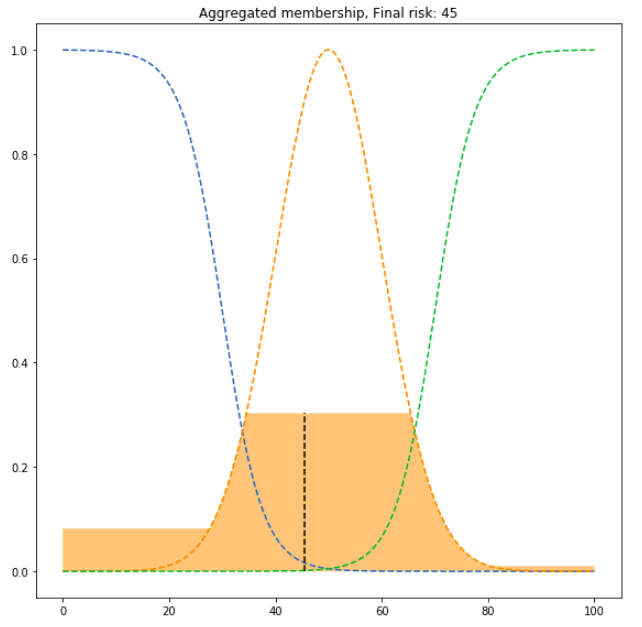
\includegraphics[width=.8\linewidth]{figures/second/prod-centroid.png}  
  \caption{Final aggregation result with the centroid method for defuzzification.}
  \label{fig:2prod-centroid}
\end{subfigure}
\begin{subfigure}{.5\textwidth}
  \centering
  % include second image
  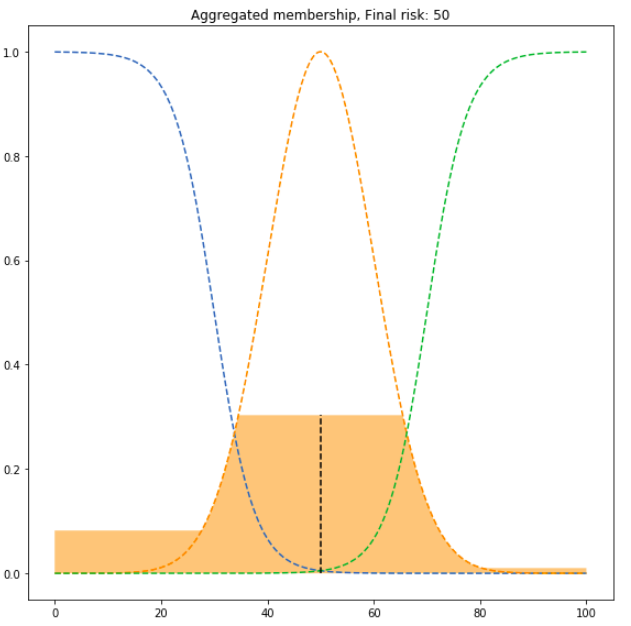
\includegraphics[width=.8\linewidth]{figures/second/prod-mom.png}  
  \caption{Final aggregation result with the mean of maximum method for defuzzification.}
  \label{fig:2prod-mom}
\end{subfigure}
\begin{subfigure}{.5\textwidth}
  \centering
  % include second image
  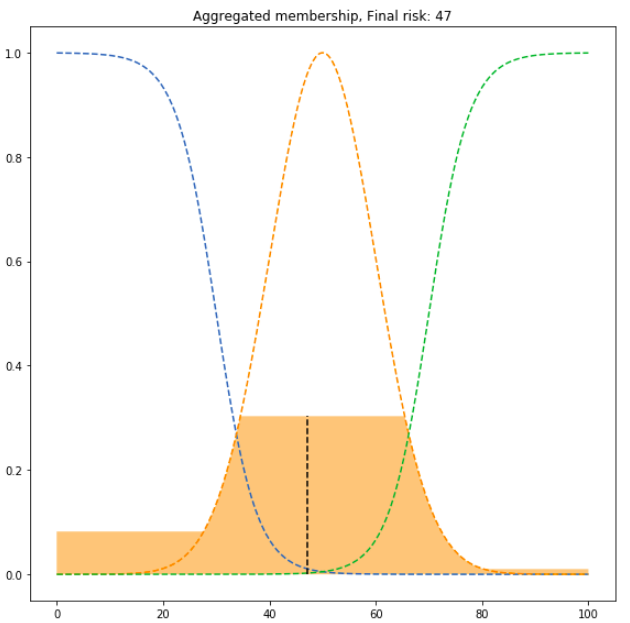
\includegraphics[width=.8\linewidth]{figures/second/prod-bisector.png}  
  \caption{Final aggregation result with the bisector method for defuzzification.}
  \label{fig:2prod-bisector}
\end{subfigure}
\caption{Results for test case 2 using the T-norm product.}
\label{fig:testcase2prod}
\end{figure*}


\subsubsection{Test case 3}
In the Figures~\ref{fig:testcase3min} and \ref{fig:testcase3prod} are shown the results for the final test case. This patient has an advanced age, however, their habits are really good, and even when their heritage is not the best, the risk of developing cancer is medium, varying between 44 and 50. In this case, the mean of maximum defuzzification produces again the highest output, and the product norm is higher than the minimum norm. Here, we identify the fact that, for the model, the habits have the same importance as the heritage, and can compensate a high age and a bad heritage.
\begin{figure*}[ht]
\begin{subfigure}{.5\textwidth}
  \centering
  % include third image
  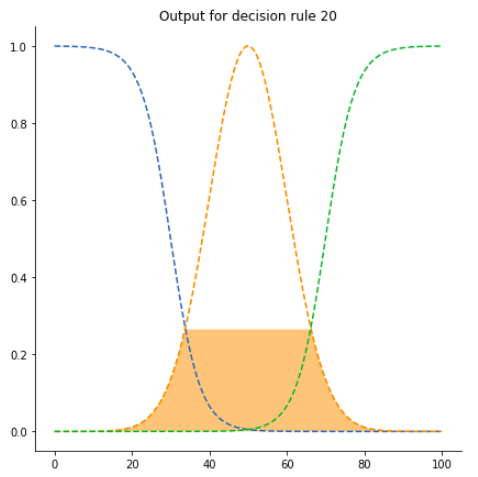
\includegraphics[width=.8\linewidth]{figures/third/min1.png}  
  \caption{Output for decision rule 20 with the T-norm minimum.}
  \label{fig:3min1}
\end{subfigure}
\begin{subfigure}{.5\textwidth}
  \centering
  % include third image
  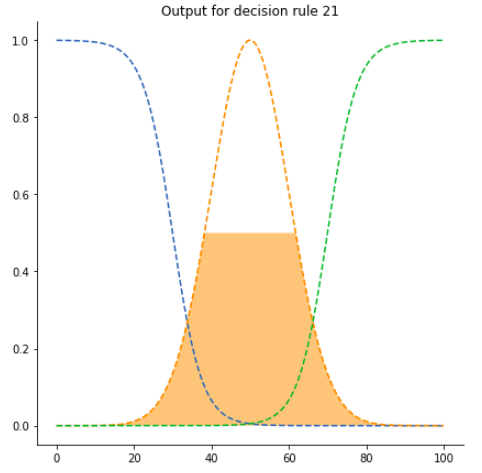
\includegraphics[width=.8\linewidth]{figures/third/min2.png}  
  \caption{Output for decision rule 21 with the T-norm minimum.}
  \label{fig:3min2}
\end{subfigure}
\begin{subfigure}{.5\textwidth}
  \centering
  % include third image
  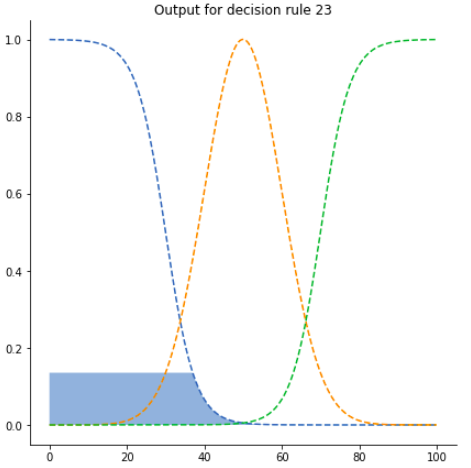
\includegraphics[width=.8\linewidth]{figures/third/min3.png}  
  \caption{Output for decision rule 23 with the T-norm minimum.}
  \label{fig:3min3}
\end{subfigure}
\begin{subfigure}{.5\textwidth}
  \centering
  % include third image
  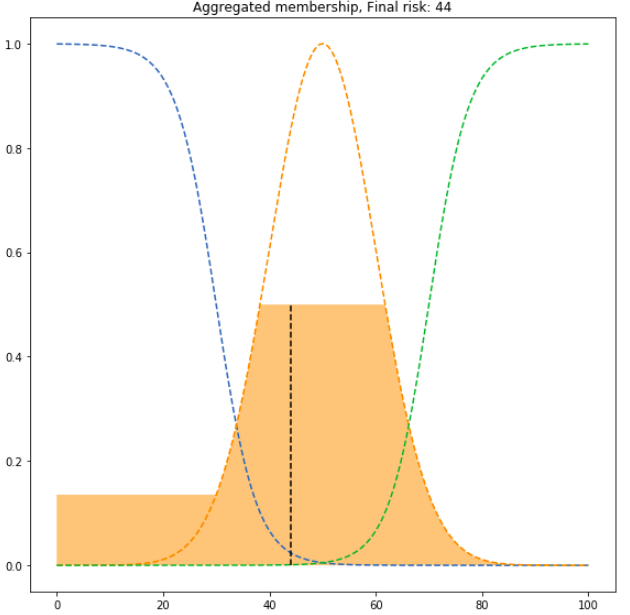
\includegraphics[width=.8\linewidth]{figures/third/min-centroid.png}  
  \caption{Final aggregation result with the centroid method for defuzzification.}
  \label{fig:3min-centroid}
\end{subfigure}
\begin{subfigure}{.5\textwidth}
  \centering
  % include third image
  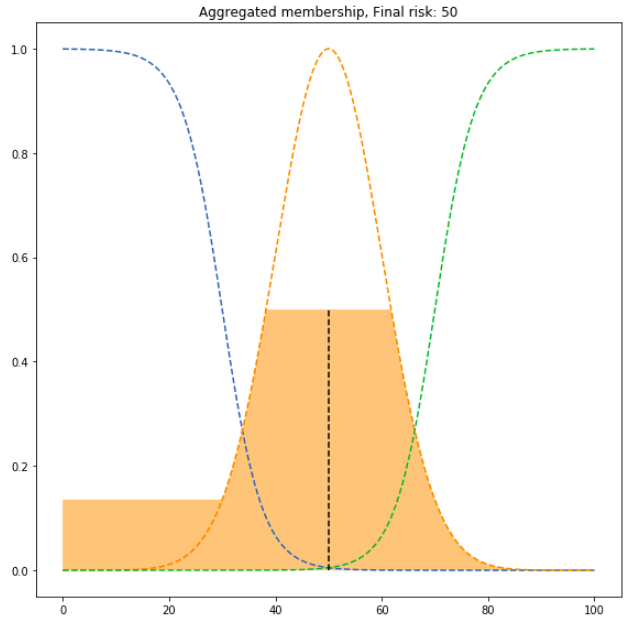
\includegraphics[width=.8\linewidth]{figures/third/min-mom.png}  
  \caption{Final aggregation result with the mean of maximum method for defuzzification.}
  \label{fig:3min-mom}
\end{subfigure}
\begin{subfigure}{.5\textwidth}
  \centering
  % include third image
  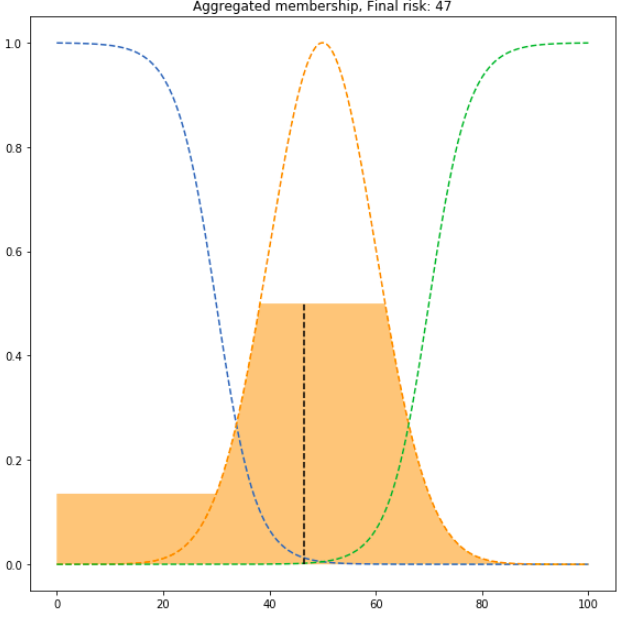
\includegraphics[width=.8\linewidth]{figures/third/min-bisector.png}  
  \caption{Final aggregation result with the bisector method for defuzzification.}
  \label{fig:3min-bisector}
\end{subfigure}
\caption{Results for test case 3 using the T-norm minimum.}
\label{fig:testcase3min}
\end{figure*}

\begin{figure*}[ht]
\begin{subfigure}{.5\textwidth}
  \centering
  % include third image
  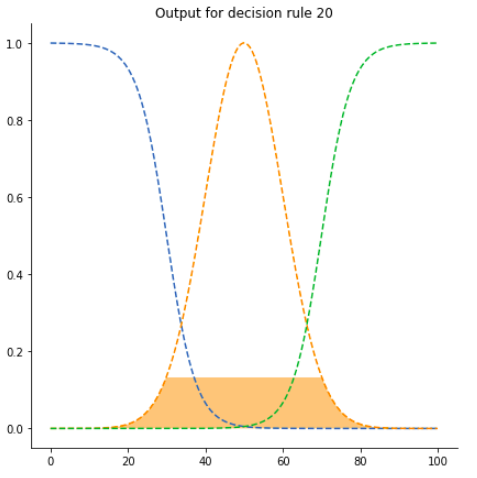
\includegraphics[width=.8\linewidth]{figures/third/prod1.png}  
  \caption{Output for decision rule 20 with the T-norm product.}
  \label{fig:3prod1}
\end{subfigure}
\begin{subfigure}{.5\textwidth}
  \centering
  % include third image
  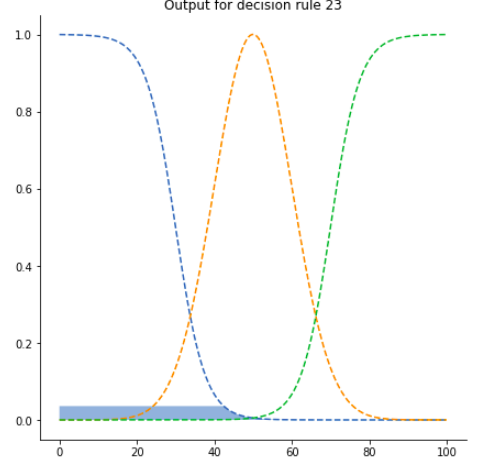
\includegraphics[width=.8\linewidth]{figures/third/prod2.png}  
  \caption{Output for decision rule 23 with the T-norm product.}
  \label{fig:3prod2}
\end{subfigure}
\begin{subfigure}{.5\textwidth}
  \centering
  % include third image
  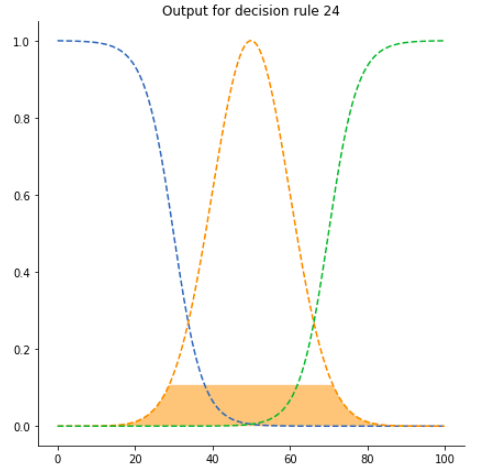
\includegraphics[width=.8\linewidth]{figures/third/prod3.png}  
  \caption{Output for decision rule 24 with the T-norm product.}
  \label{fig:3prod3}
\end{subfigure}
\begin{subfigure}{.5\textwidth}
  \centering
  % include third image
  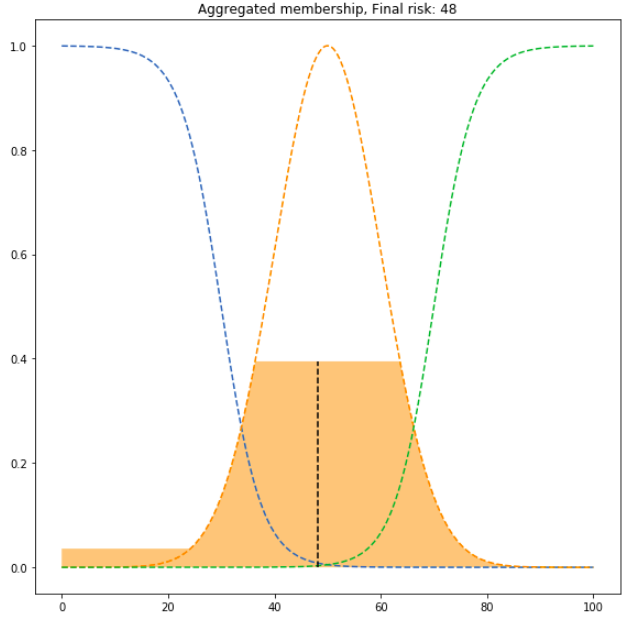
\includegraphics[width=.8\linewidth]{figures/third/prod-centroid.png}  
  \caption{Final aggregation result with the centroid method for defuzzification.}
  \label{fig:3prod-centroid}
\end{subfigure}
\begin{subfigure}{.5\textwidth}
  \centering
  % include third image
  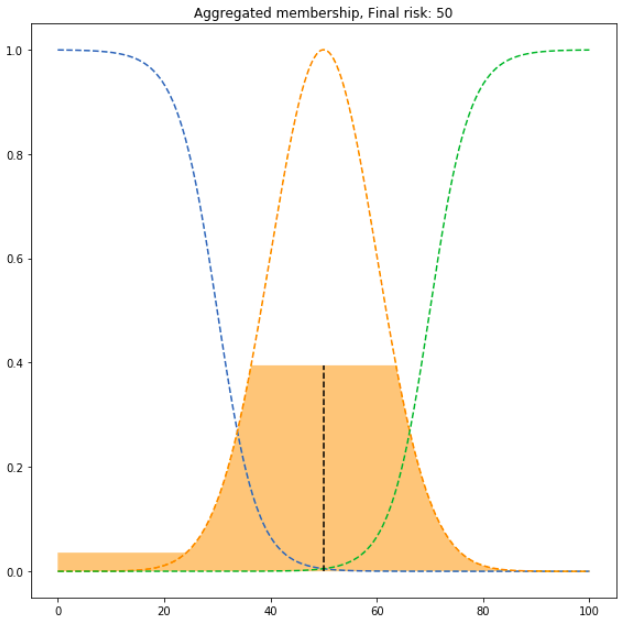
\includegraphics[width=.8\linewidth]{figures/third/prod-mom.png}  
  \caption{Final aggregation result with the mean of maximum method for defuzzification.}
  \label{fig:3prod-mom}
\end{subfigure}
\begin{subfigure}{.5\textwidth}
  \centering
  % include third image
  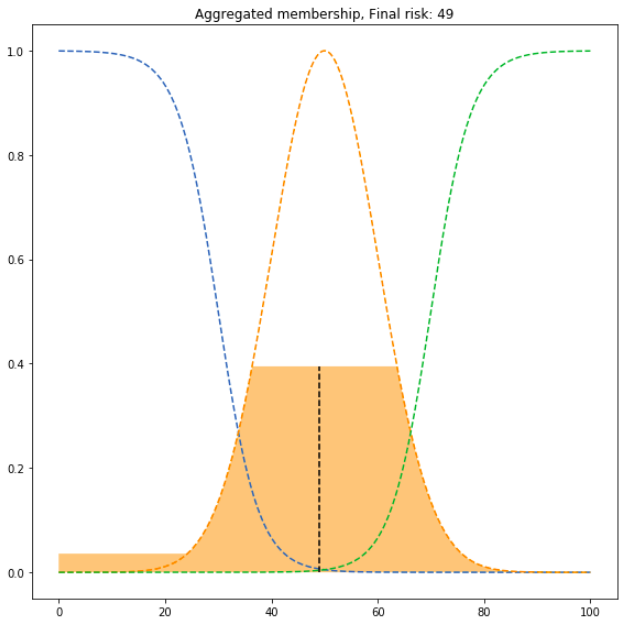
\includegraphics[width=.8\linewidth]{figures/third/prod-bisector.png}  
  \caption{Final aggregation result with the bisector method for defuzzification.}
  \label{fig:3prod-bisector}
\end{subfigure}
\caption{Results for test case 3 using the T-norm product.}
\label{fig:testcase3prod}
\end{figure*}


\section{Conclusions}


\nocite{*}
\bibliography{ref}
\bibliographystyle{IEEEtran}


\end{document}
